% TODO FOR NEXT YEAR
% - TODO: PPT-based videos that show how lists/queues/stacks work
% (transitions with smoothing effects like dissolve or 
% venetian blinds so that things "appear" or "disappear") -> probably also needed all along
% the way since the moment we start talking about simple and complex types. 
%
% - TODO: check than in Java7 you can switch/case with Strings

\section{Static data}
\label{sec:static-data}

There are few Java keywords that we do not know yet. One of them is
\verb+static+. This keyword means that the field or method that comes
after it does not belong to an object of a class but to the class
itself: it is a class member rather than an object member\footnote{The
name \emph{static} is a bit confusing at first, because it does not
mean that static things do not move but rather that they belong to the
class and not its instances (i.e.~objects). It may have been better to
use a keyword like \emph{class}, but it is already used to define
classes themselves.}.

Why would we be interested in using \verb+static+? 

\paragraph{Static fields}
\label{sec:static-fields}

There is little use for static fields. There are few cases in which
some information of our objects should not be stored in the objects
themselves but in the class, and it is common that this information is
constant. For example, we could store the number of chromosomes of an
animal: this information does not change from animal to animal:

\begin{verbatim}
    public class Human {
        private static chromosomeCount;
        private String name;
        private int age;
        // ...
    }
\end{verbatim}

Every human has a different name and a different age, but the same
number of chromosomes. Making it \verb+static+ makes it clear to other
programmers with little knowledge of biology that the chromosome count
is the same for all humans\footnote{For the sake of simplicity, we
  ignore in this example chromosomical conditions such the Down,
  Patau, Turner, and Klinefelter syndromes.}. 

It also saves a little
memory because 
the variable is stored only once (in the class) rather than many times
(once per object). For every name, there is one and only one static
variable per class per machine; in other words, there is only one
\verb+chromosomeCount+ in class \verb+Human+ in the whole
computer\footnote{Being precise, there is only one per \emph{Java
    Virtual Machine} (JVM). There may be more than one JVM in a
  physical computer, although this is not relevant in most cases and
  the ``there is one static X per machine'' is mostly true.}. 

% NOTE: 
% I introduce here the example of counting objects of a class for two
% reasons: 
% 
%  - It is the example you find EVERYWHERE. For me, this is a good
%   indication that static fields have little use apart from
%   constants (the other pervasive example, but I do not want to
%   introduce "final" yet... one keyword per day)... So if my
%   students look this up in another book, it will sound familiar. 
%  - It is a use case with a little actual validity if you think in
%   terms of n-singletons and factories. 
% 
% These two are the only arguments. If they become invalid in the
% future, then the example should be removed. 

You can use a static variable to keep a counter of how many objects of
a class have been created, as in the example: 

\begin{verbatim}
    public class Spy {
        private static int spyCount = 0;

        public Spy(...) {
            spyCount++;
            // ...
        }

        public static int getNumberOfSpies() {
            return spyCount;
        }
        // ...
    }
\end{verbatim}

Every time the constructor of \verb+Spy+ is called (using \verb+new+) 
the counter \verb+spyCount+ is
increased; we could also think of a \verb+die()+ method that reduces
the counter. In any case, it is rarely necessary to keep a count of
objects of a class, and therefore static variables are seldom used
except as constants. 

\paragraph{Static methods}
\label{sec:static-methods}

Static methods are class methods. They do not need to be called from
an object, but can be called directly from the class. You have already
seen some examples as \verb+Math.random()+ 
and the widely used \verb+Integer.parseInt(String)+. 

Static methods can only access \verb+static+ fields. As they are
run from the \emph{class}, they can only access data that is \emph{in the class} and
not \emph{in the objects}. You can think of it in the following way: the
class does not know where the objects are stored in the memory, so
all instance data (i.e.~data in the objects) cannot be accessed. Class data and
class methods, however, can be accessed from anywhere, just using the
name of the class (as in \verb+Integer.parseInt(String)+). 

\paragraph{Rules of thumb}
\label{sec:rules-thumb-use}

It is important to understand what \verb+static+ means in Java,
because you will find this keyword quite often in your life as a Java
programmer. On the other hand, it is a keyword that you will not use
that much; and when you do, it will be almost always in one of three
situations as explained below. 

In other words, if you had to remember just four things about the keyword
\verb+static+, remember these four rules: 

\begin{itemize}
\item Use \verb+static+ \emph{sparingly}. If you use it often, you are
  probably doing it wrong. Thing again about your program, and look
  for ways to get rid of your static state (i.e.~fields/variables).
\item If you have static fields, they should be \emph{constants} and they
  should be \verb+public+. One such example is \verb+Math.PI+: its
  value is always the same 3,14159\ldots
\item If you have static methods, they should be \emph{pure functions}. This
  means they should not have side effects, and they should return a
  value that depends only on their arguments. One such example is
  \verb+Integer.parseInt(String)+.
\item If you have a \verb+main+ method, it must be static as there is
  only one per class (at most). 
\end{itemize}

What is the \verb+main+ method? I am glad you asked. The \verb+main+
method is the entry point for your Java application. 

\section{The main method}
\label{sec:main-method}

As we leave Groovy and Java Decaf behind and move into full-flavour Java, we need a
way to launch our program: a starting point. It is all too well to
have a lot of Java classes, each of them in their own \verb+.java+
file, but this is of little use if we cannot start our program from
the command like (or clicking on an icon, for that matter). 

In Groovy and Java Decaf, we did not need an entry point. The programs or scripts
were their own entry point. For example, we only needed to 
write \verb+groovy myScript.groovy+ and Groovy would
start the execution. The situation is slightly more complex in Java
because all files are classes, not scripts. We need to have an entry
point, a place in the code where Java knows that the execution of the
program can start. This entry point is the \verb+main+ method. The
main method is a method like any other, and every class can have
one. It looks like this:

\begin{verbatim}
    public static void main(String[] args) {
      // Here be the code to launch the program
    }
\end{verbatim}

If a class has a main method, it can be run from the operating system
by typing: 

\begin{verbatim}
    > java myClass
\end{verbatim}

assuming that there is a \verb+myClass.class+ file. The 
signature of the \verb+main+ method is a bit long, but we have
already learnt what each of its elements means: 

\begin{itemize}
\item It must be \verb+public+, because otherwise it cannot be
  accessed from outside the class (and how would the program launch
  then?).
\item It must be \verb+static+, because it pertains to the class, not
  to each of its instances (i.e.~objects).
\item It returns \verb+void+. This is a method that is never called by
  other classes, so a return type is unnecessary.
\item The only parameter is a 1-D array of Strings, called \verb+args+
  (short for arguments). Actually the name is not important. The
  elements in the array are the parameters passed in the command line,
  if any. For example, if you run a program with a line like
  \verb+java myClass+ \verb+www.google.com+ \verb+80+ \verb+true+, 
  the first element
  of \verb+args+ (i.e.~args[0]) will be ``www.google.com'', 
  the second element (i.e.~args[1]) will be ``80'', 
  and the third one (i.e.~args[2]) will be ``true''. All of them are
  Strings, if you
  want to use these parameters with a different type you need to parse
  them. 
\end{itemize}

\subsection*{Liberating your main method from static restrictions}
\label{sec:liber-your-launch}

As static code does not understand anything about instance
(i.e.~non-static) methods or data, you will not be able to use your
instance data in your main method. This seems restricting at first,
as in the following example: imagine that we want to start a program
from a BitTorrentDownloader class, and we want to give the name of the
host and the port from the command line

\begin{verbatim}
    public class BitTorrentDownloader {
        private String host;
        private int port;
    
        public BitTorrentDownloader(String host, int port) {
            this.host = host;
            this.port = port;
        }
    
        public static void main(String[] args) {
            host = args[0];
            port = Integer.parseInt(args[1]);
            // with the fields initialised, 
            // launching code comes here...
            // ...
        }
    }
\end{verbatim}

When you try to compile this program, java will complain with the
following error: 

\begin{verbatim}
    non-static variables cannot be referenced from a static context
    host = args[0];
    ^
    port = Integer.parseInt(args[1]);
    ^
\end{verbatim}

One (bad) solution is to make \verb+host+ and \verb+port+ static, but
that means that there can only be one of each. This is usually a bad
idea in the long run. Maybe in a future version you will like several
BitTorrentDownloaders working in parallel, or maybe you would to
launch many at the same time and put them in a queue. All of this
would be impossible if the fields were static. Remember: \verb+static+
means ``only one per class'', and programmers usually like to have as
many as possible of everything, just in case. As a rule of thumb,
\textbf{never make anything ``static'' unless it is absolutely necessary}.

There is another (much better) solution: to instantiate the class
inside its own main method, and then run all the code from a non-static
launching method. This method is commonly called \verb+run()+ or
\verb+launch()+. See the example: 

\begin{verbatim}
    public class BitTorrentDownloader {
        private String host;
        private int port;
    
        public BitTorrentDownloader(String host, int port) {
            this.host = host;
            this.port = port;
        }
    
        public static void main(String[] args) {
            // 1. Parameter analysis / processing
            String host = args[0];
            int port = Integer.parseInt(args[1]);
            // 2. Object construction / building of main data structures
            BitTorrentDownloader downloader = new BitTorrentDownloader(host, port);
            // 3. Execution of the program
            downloader.launch();
        }

        private void launch() {
            // with the fields initialised, 
            // launching code comes here...
            // ...
        }
    }
\end{verbatim}

As you can see the main method is very simple and has only three
parts: parameter analysis, creation of the main structures, and
starting the execution of the program. It is a good idea to follow
this structure in every main method. This will keep your main methods
simple and to the point. If you notice that your main methods are
getting longer than a few lines, make a pause, take a deep breath, and
think things through again. 

\section{More differences between Groovy and Java}
\label{sec:more-diff-betw}

\subsection{String.equals() != ==}
\label{sec:string.equals-=-==}

In Groovy we have become used to comparing String using ``==''. In
Java we have to be careful and use the method
\verb+.equals()+. Otherwise we may get funny results like in the
following simple code: 

\begin{verbatim}
    System.out.print("Enter a string: ");
    String str1 = System.console().readLine();
    System.out.print("Enter another string: ");
    String str2 = System.console().readLine();
    System.out.println("Are '" + str1 + "' and '" + str2 + "' the same?");
    System.out.println("Using ==: " + (str1 == str2));
    System.out.println("Using .equals(): " + (str1.equals(str2)));
\end{verbatim}

that produces the following output: 

\begin{verbatim}
    Enter a string: This is a String
    Enter another string: This is a String
    Are 'This is a String' and 'This is a String' the same?
    Using ==: false
    Using .equals(): true
\end{verbatim}

This is because the equality operator ``=='' only works with simple
types in Java, with little ``boxes''. When it is used to compare objects like
Strings, it compares the pointers not the contents of the objects (see
Figure~\ref{fig:equals}). The
method \verb+.equals()+, on the other hand, can be used to compare the
content of the objects. 

\begin{figure}[bthp]
  \centering
  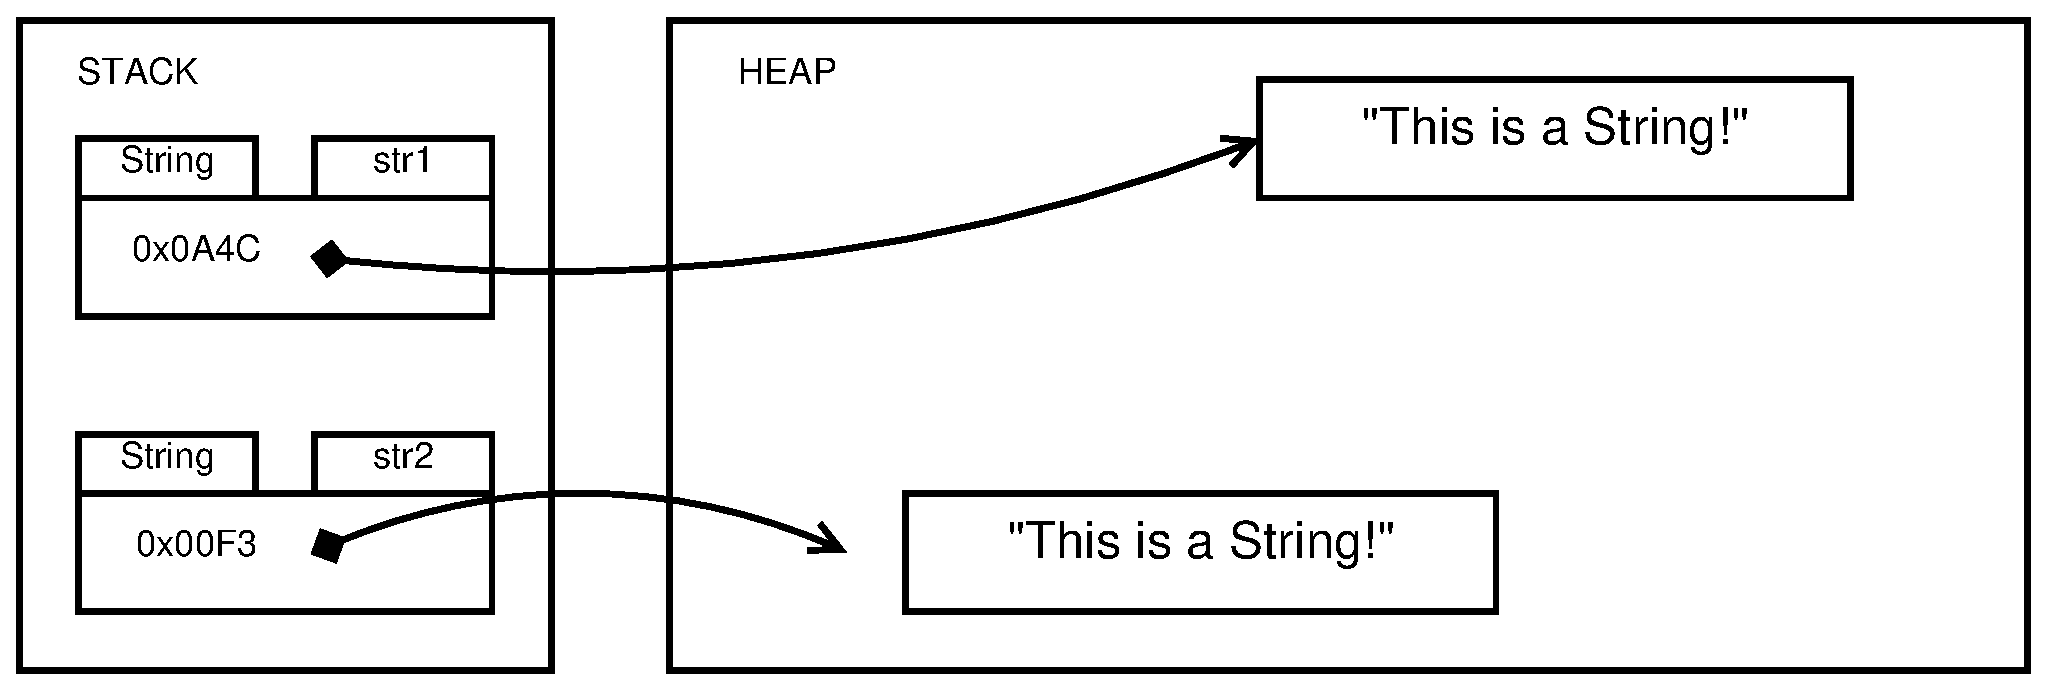
\includegraphics[width=\textwidth]{gfx/variables-string-equals}
  \caption{The operator ``=='' compares simple types. When used to
    compare complex types, it compares just the pointers. Strings str1
  and str2 have the same content but their pointers are different,
  i.e.~they point to different memory addresses.} 
  \label{fig:equals}
\end{figure}

As a rule of thumb, \textbf{always use the method .equals()
  when comparing Strings} or any other complex types in Java.

\paragraph{Note.}
\label{sec:notre}

For some classes, the effect of \verb+.equals()+ is the same as
``=='', i.e.~it compares the pointers and not the content of the
objects. This depends on the class and its semantics. For instance,
we usually think that two Strings or two Integers (class, not simple
type) are the same if they have the same value, but we do not think
of two \verb+Person+ to be same even if they have the same name. We
will learn more about this when we learn about class inheritance but,
for now, it suffices to say that objects should always be compared
with \verb+equals()+ and not with ``==''. The operator ``=='' should
only be used for simple types (also known as \emph{primitive} types). 

\subsection{A new type of loop: do\ldots while}
\label{sec:new-type-loop}

With a loop you can perform the same operations over and over
again. However, if the condition for the loop is never true a
\texttt{while} loop will never run; and sometimes you need it to run
at least once, like in this case:

\begin{verbatim}
    System.out.println("Enter the names of your friends. Finish by typing END.");
    String name = System.console().readLine();
    System.out.println(name + ": friend");
    while (!name.equals("END")) {
        System.out.println(name + ": friend";
        name = System.console().readLine();
    }
\end{verbatim}

In this brief example you need to repeat the same code to read input
from the user in two different places. If
the only way to do loops was using \texttt{while}, this repetition
could not be avoided (and in a less trivial program, with
intelligent error-checking and the like, this could be a lot of
repetition!). Fortunately, in Java we can use 
the \texttt{do\ldots while} loop: 

\begin{verbatim}
    System.out.println("Enter the names of your friends. Finish by typing END.");
    String name;
    do {
        name = System.console().readLine();
        System.out.println(name + ": friend");
    } while (!name.equals("END"));
\end{verbatim}

Note that you must declare the string \verb+name+ before the loop
starts. Otherwise, you cannot make checks on it at the end of the loop
because it would have been out of scope and forgotten by the
computer. 

Remember, repeated code is usually a bad sign: a symptom of poor
design and/or poor programming. When you have the same code in two
different places, and make a change in one of them, it is very easy to
forget to change the other too\ldots a common source of bugs for
careless programmers. If you notice you have repeated code in your
program, think twice about a better way of doing things, without
repetition. Remember the DRY principle: \textbf{Don't Repeat
  Yourself}. Keep it in mind at all times.

%
%
% TODO: provide rules of thumb of when to use do...while and
%       when to use while and when to use for
%
%
%
%

\subsubsection*{Exercise}

Make a class that implements a method 
that reads a list of marks between 0 and 100 from the
user, one per line, and stops when the user introduces a -1. The
program should output at the end (and only at the end) how many marks
there were in total, how many were distinctions (70--100), how many
were passes (50--69), how many failed (0--49), and how many were
invalid (e.g. 150 or -3). Use \texttt{readLine()} exactly once.

\section{Beyond arrays: lists, stacks, queues}
\label{sec:beyond-arrays:-lists}

We have seen what to do when we want to store a lot of data of the
same type: we create an array, and then store all elements
side-by-side in memory. Arrays are convenient because they store a lot
of information of the same type without 
the need to use a lot of variables. Their main disadvantage is that we
need to now the lenght of the array in advance and it cannot be
changed afterwards. 

Most applications in the real world, however, do not know in advance
how much data they will need: a hospital does not know how many
patient records it will need every day, a car manufacturer does not
know in advance how many employees it will have or how many cars it
will be producing at the same time. Even if they knew, these
desired characteristics of the program ---called
\emph{requirements}--- may change over the life of the program, e.g.~:
maybe the hospital knows it only has ninety beds, but five years later
they receive funding from the Government to extend to another building
and duplicate their capacity. A real program needs to be able to
handle arbitrary amounts of data. 

This is done by means of \emph{dynamic} data structures. The most basic
examples are lists. Stacks and queues are special types of lists. 

\subsection{Lists}
\label{sec:lists}

Dynamic lists are composed of a sequence of complex types in memory,
linked by their pointers. In other words, every element in a dynamic
list contains one element of information of a certain type (which may
be complex) and a pointer to the next element. Let's use the hospital
above to see an example. For the sake of simplicity, we can assume
that the hospital only stores three pieces of data about each patient:
name, age, and illness. The file \verb+Patient.java+ may be similar to:

\begin{verbatim}
    public class Patient {
        private String name;
        private int age;
        private String illness;
        // methods like constructors, getters 
        //   and setters come here...
    }
\end{verbatim}

And the hospital program (a different file to \verb+Patient.java+)
could have an array of patients:  

\begin{verbatim}
    Patient[] patientArray = new Patient[90];
\end{verbatim}

But, as we already know, this is limited because the hospital may have
more than 90 patients. We can overcome this limitation by using a
linked list. Our list will be composed of objects of a slightly
modified class \verb+Patient+:

\begin{verbatim}
    public class Patient {
        private String name;
        private int age;
        private String illness;
        private Patient nextPatient;

        public Patient(String name, int age, String illness) {
            this.name = name;
            this.age = age;
            this.illness = illness;
            this.nextPatient = null;
        }
        //  other methods come here...
    }
\end{verbatim}

The only difference is the pointer to another \verb+Patient+. A linked
list of patients is nothing more than a sequence of patients in which
each patient links to the next one, and the last one 
points to \verb+null+. The beginning of the list will
appear in your main program and probably be initialised in the
\verb+launch()+ method, while new patients can be added to the list by
using the following method: 

\begin{verbatim}
    // this is a member method of class Patient
    public void addPatient(Patient newPatient) {
        if (this.nextPatient == null) {
            // this means this is the last patient in the list
            this.nextPatient = newPatient;
        } else {
            this.nextPatient.addPatient(newPatient);
        }
    }            
\end{verbatim}

The method \verb+addPatient(Patient)+ is very simple. It goes through
the whole list of patients checking whether the current patient is the
last one in the list (\emph{this.nextPatient == null}). 
If it is, it adds the last patient at the
end; if it is not, it moves to the next patient and tries 
again (\emph{this.nextPatient.addPatient(newPatient)}). 

The list of patients is initialised in the main program with a first
patient, as shown in the code below (see also Figure~\ref{fig:jkhsdfj}):

\begin{verbatim}
    public class HospitalManager {
        private Patient patientListStart = null;

        public static void main(String[] args) {
           // ...
           HospitalManager hm = new HospitalManager();
           // ...
        }

        // ...inside some method, maybe launch()
            Patient firstPatient = new Patient("John", 33, "Tuberculosis");
            patientListStart = firstPatient;
        // ...
    }
\end{verbatim}

% TODO: put the full diagram (with the init of the list in the heap,
% since it is in an object) as a end-of-book-note. 

\begin{figure}[bthp]
  \centering
  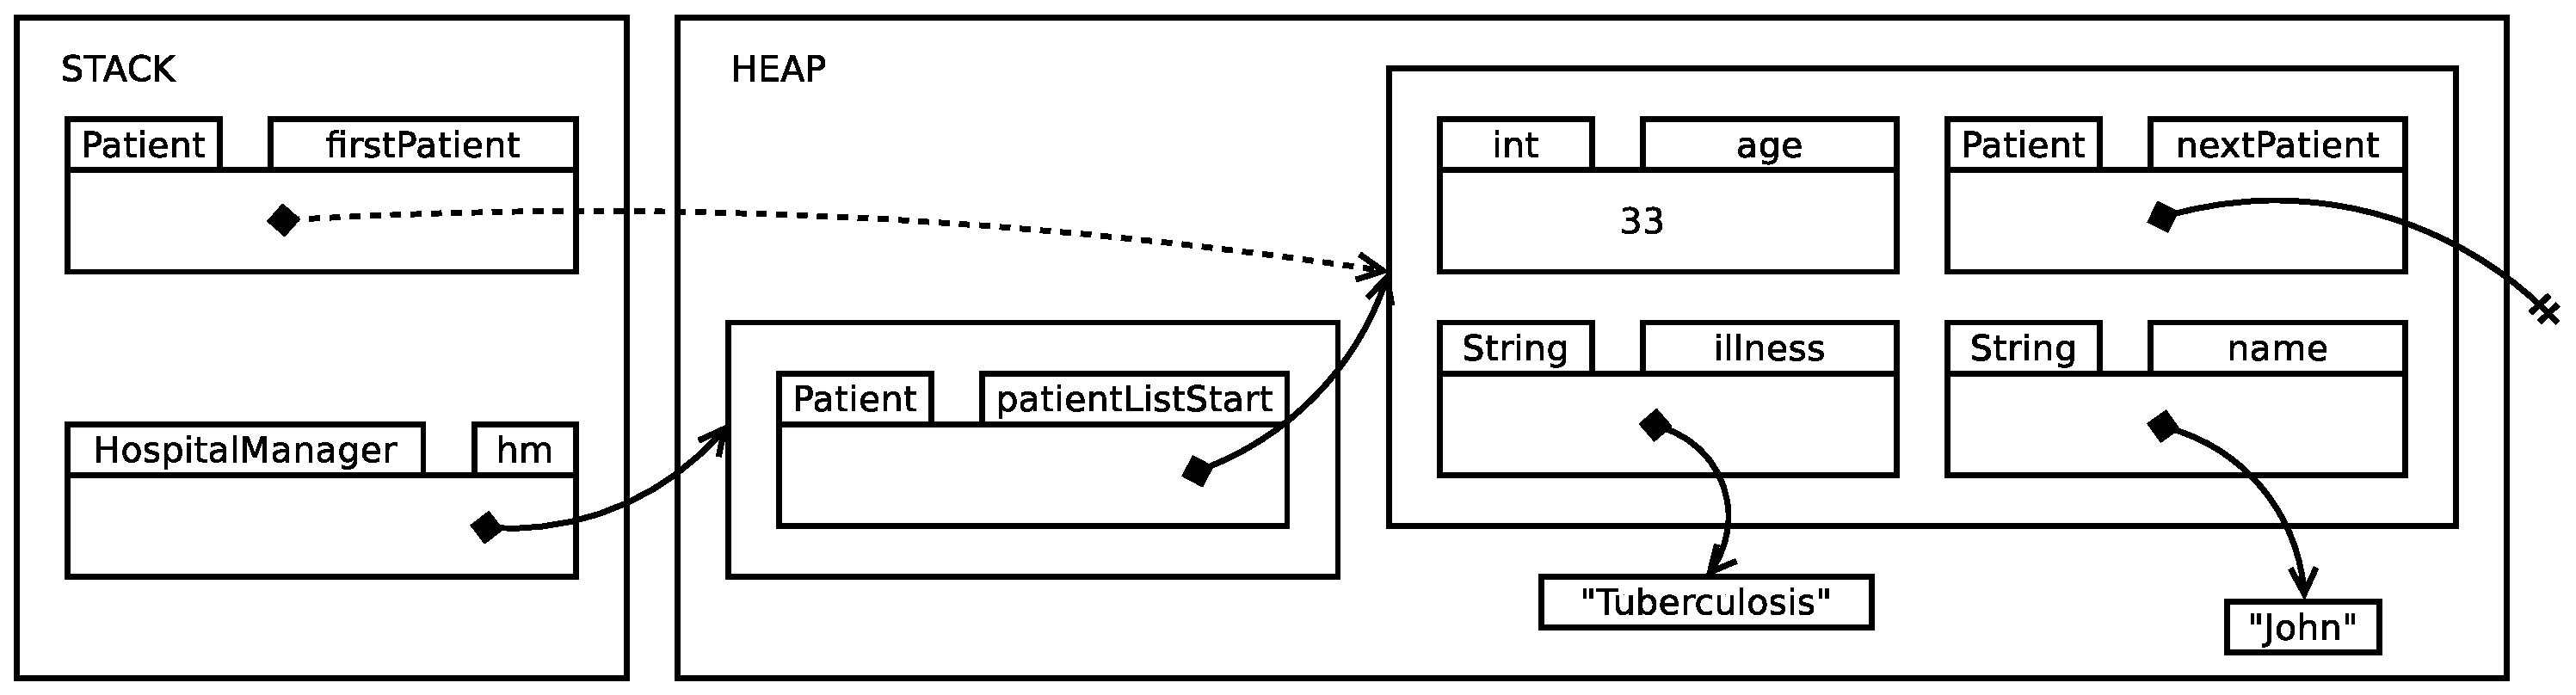
\includegraphics[width=\textwidth]{gfx/lists-init-full}  
  \caption{In order to initialise the list, we create a Patient and
    point the initial pointer (patientListStart) to it. At the end of
    the method, the pointer firstPatient is forgotten but the list
    remains linked from patientListStart.}
  \label{fig:jkhsdfj}
\end{figure}

From then on, new patients can be added by calling the
method \verb+addPatient(Patient)+ at any point. 

\begin{verbatim}
    Patient yetAnotherPatient = new Patient("Mary", 66, "Meningitis");
    patientListStart.addPatient(yetAnotherPatient);
\end{verbatim}

%% TODO: a ppt video about this? an activity in the class?

Patients can also be removed easily from the list. The program must be
careful not to leave any pointers loose to prevent information
loss. For example, a method to remove patients by name would look like
this (see also
Figures~\ref{fig:deletelinklist},~\ref{fig:deletelinklist2},
and~\ref{fig:deletelinklist3}):

\begin{verbatim}
    // this is a member method of class Patient
    // returns true if the patient was found and removed, false otherwise
    public boolean deletePatient(Patient patient) {
        if (this.nextPatient == null) {
            // patient to remove was not found
            return false;
        } else if (this.nextPatient.name.equals(patient.name)) {
            // We found it! It is the next one!
            // Now link this patient to the one after the next 
            this.nextPatient = nextPatient.nextPatient;
            return true;
        } else {
            return this.nextPatient.deletePatient(patient);
        }
    }    
\end{verbatim}

\begin{figure}[p]
  \centering
  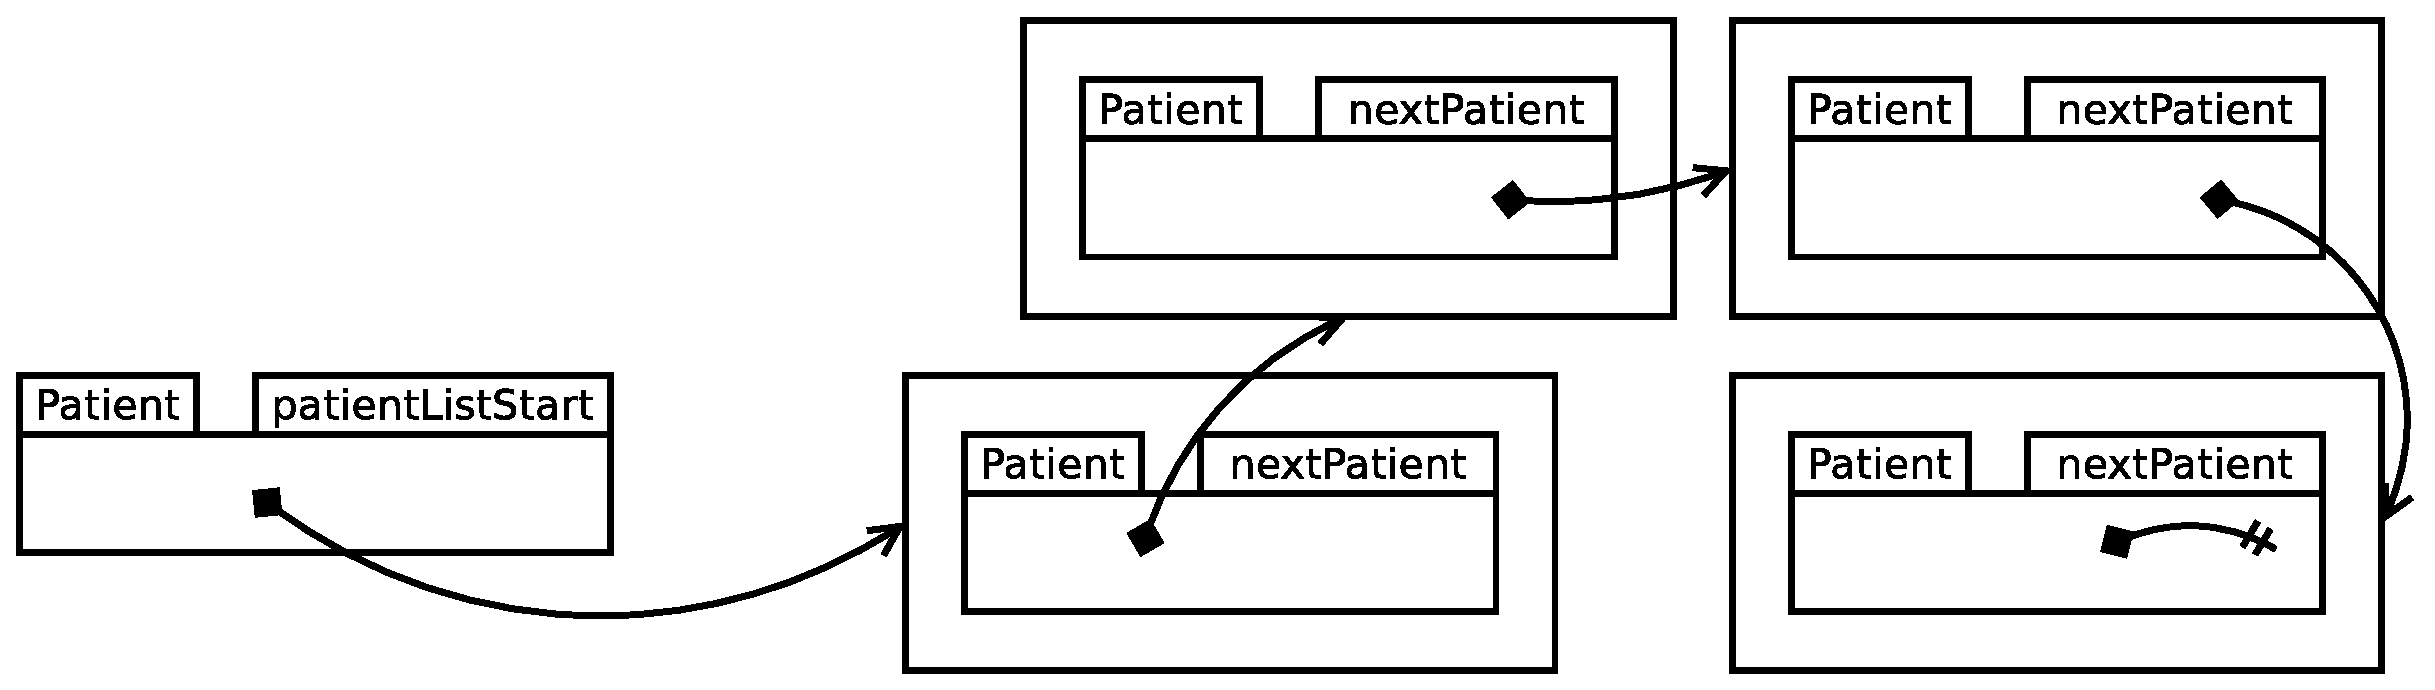
\includegraphics[width=14cm]{gfx/lists-remove-1}    
  \caption{Deletion of elements in a linked list, step one: finding
    the element we want to delete. Suppose that we want to delete the
    second elements in the list. In order to delete it from the list
    of patients, we must link the 
    former patient to the following patient. 
    (Note: simplified diagram.)}
  \label{fig:deletelinklist}
\end{figure}

\begin{figure}[p]
  \centering
  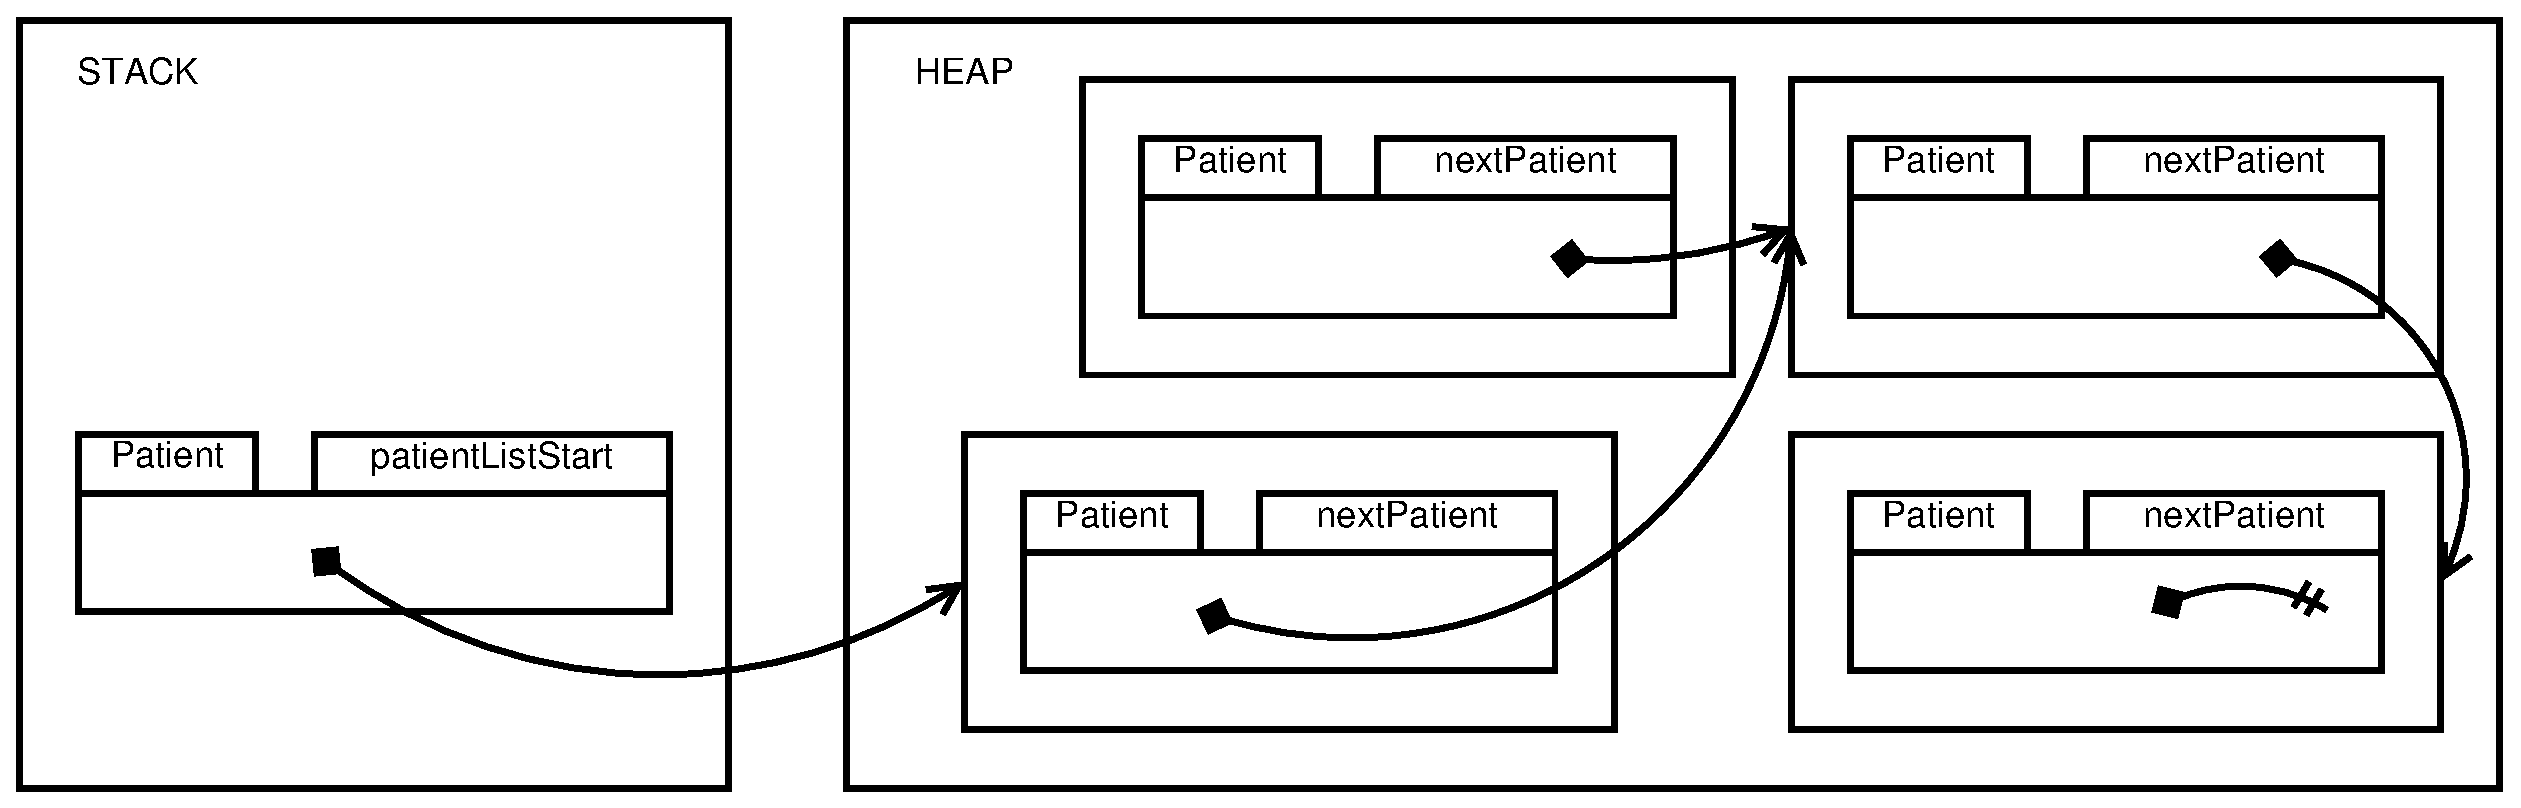
\includegraphics[width=14cm]{gfx/lists-remove-2}    
  \caption{Deletion of elements in a linked list, step two: linking
    the former patient to the following patient. 
    (Note: simplified diagram.)}
  \label{fig:deletelinklist2}
\end{figure}

\begin{figure}[p]
  \centering
  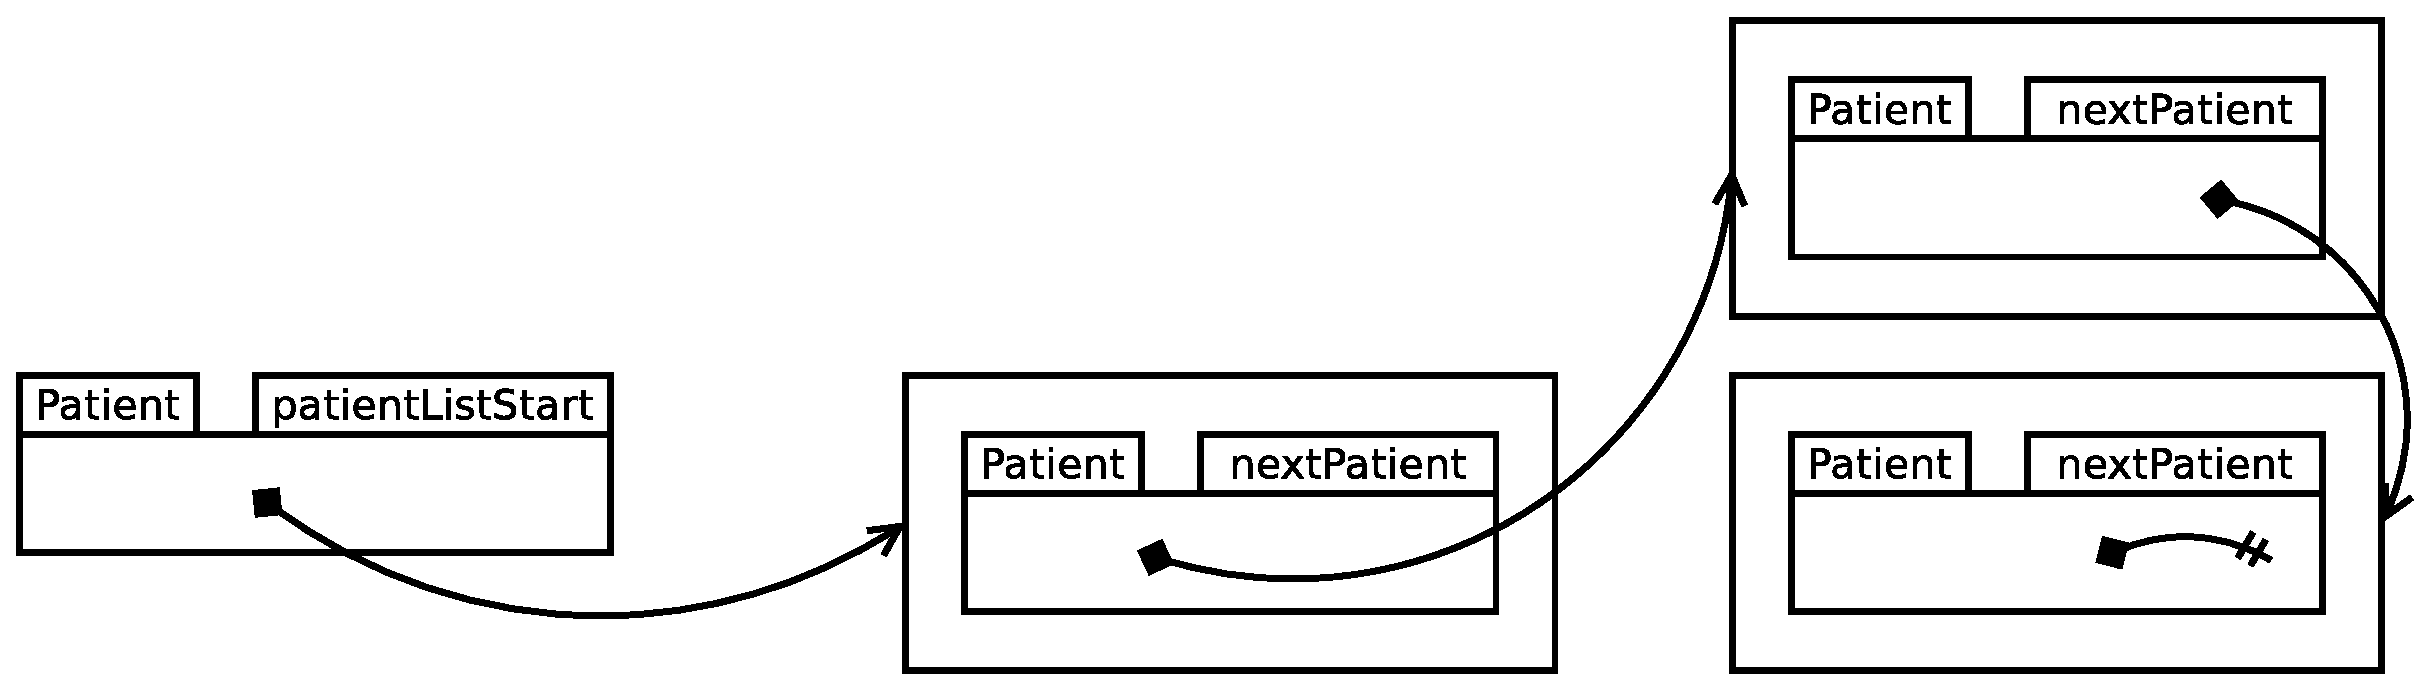
\includegraphics[width=14cm]{gfx/lists-remove-3}    
  \caption{Deletion of elements in a linked list, step three: 
    The deleted patient's memory will be collected automatically by
    Java's garbage collector. The memory is then free to be used by
    other objects.
    (Note: simplified diagram.)}
  \label{fig:deletelinklist3}
\end{figure}

When we delete an element from a dynamic linked list, it is left
``hanging around'' without any pointer that links to it. This will be
detected automatically by Java and the object will be destroyed in a
process called \emph{garbage collection} 
(Figure~\ref{fig:deletelinklist3}). The memory freed in this
process can then be used to create other objects in the heap. We will
learn more about how garbage collection works in the future. % TODO:
                                % write this. 





%%% Local Variables:
%%% mode: latex
%%% TeX-master: "main"
%%% End:
